\documentclass[aspectratio=169]{beamer}

\usepackage{iftex}
\ifPDFTeX
  \usepackage[utf8]{inputenc}
  \usepackage[T1]{fontenc}
\else
  \usepackage{fontspec}
  \IfFontExistsTF{DejaVu Sans}{
    \setsansfont{DejaVu Sans}
    \setmainfont{DejaVu Sans}
  }{
    \setsansfont{Arial}
    \setmainfont{Arial}
  }
  \IfFontExistsTF{Consolas}{
    \setmonofont{Consolas}
  }{
    \setmonofont{Courier New}
  }
\fi
\usepackage[czech]{babel}
\usepackage{graphicx}
\usepackage{booktabs}
\usepackage{array}
\usepackage{tikz}
\usetikzlibrary{positioning}

\usetheme{Madrid}
\usecolortheme{default}
\setbeamertemplate{navigation symbols}{}
\setbeamertemplate{footline}[frame number]

\definecolor{TrackerGreen}{RGB}{42,118,96}
\definecolor{TrackerGray}{RGB}{90,90,90}
\setbeamercolor{structure}{fg=TrackerGreen}
\setbeamercolor{title}{fg=white,bg=TrackerGreen}
\setbeamercolor{frametitle}{fg=white,bg=TrackerGreen}
\setbeamercolor{palette primary}{fg=white,bg=TrackerGreen}
\setbeamercolor{palette secondary}{fg=white,bg=TrackerGreen}
\setbeamercolor{palette tertiary}{fg=white,bg=TrackerGreen}
\setbeamercolor{title in head/foot}{fg=white,bg=TrackerGreen}
\setbeamercolor{author in head/foot}{fg=white,bg=TrackerGreen}
\setbeamercolor{date in head/foot}{fg=white,bg=TrackerGreen}
\setbeamercolor{normal text}{fg=TrackerGray}

\title[Vývoj mobilní aplikace]{Vývoj mobilní aplikace}
\subtitle{Záznam fyzické aktivity}
\author{Jaroslav Radimský}
\date{3. června 2026}

\newcommand{\phoneshot}[2]{%
  \begin{figure}
    \centering
    \includegraphics[height=#1]{#2}
  \end{figure}
}

\begin{document}

\begin{frame}
  \titlepage
\end{frame}

\begin{frame}{Cíl řešení}
  \begin{itemize}
    \item Vytvořit samostatnou Android aplikaci pro záznam fyzické aktivity.
    \item Ukládat záznamy aktivity do lokální databáze.
    \item Zobrazit historii měření a detailní statistiky.
  \end{itemize}
\end{frame}

\begin{frame}{Hlavní obrazovka}
  \begin{columns}[T,onlytextwidth]
    \begin{column}{0.42\textwidth}
      \phoneshot{0.73\textheight}{screenshots/01-main.png}
    \end{column}
    \begin{column}{0.55\textwidth}
      \begin{itemize}
        \item První spuštění zobrazuje prázdnou historii měření.
        \item Stavový text ukazuje počet záznamů nebo informaci, že zatím žádné měření neexistuje.
        \item Tlačítko \textit{Zahájit aktivitu} otevírá samostatnou obrazovku měření.
      \end{itemize}
    \end{column}
  \end{columns}
\end{frame}

\begin{frame}{Průběh měření}
  \begin{columns}[T,onlytextwidth]
    \begin{column}{0.42\textwidth}
      \begin{figure}
        \centering
        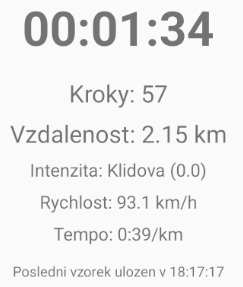
\includegraphics[width=0.9\linewidth]{screenshots/activity_cropped.png}
      \end{figure}
    \end{column}
    \begin{column}{0.55\textwidth}
      \begin{itemize}
        \item Samostatná celoplošná aktivita zobrazuje běžící čas.
        \item Aplikace ukazuje kroky, vzdálenost, intenzitu, rychlost a tempo.
        \item Vzorky se ukládají pravidelně po pěti sekundách.
      \end{itemize}
    \end{column}
  \end{columns}
\end{frame}

\begin{frame}{Notifikace běžící aktivity}
  \begin{figure}
    \centering
    
\includegraphics[width=0.82\textwidth]{screenshots/05-notification-running-crop.png}
  \end{figure}
  \begin{itemize}
    \item Při měření se zobrazuje průběžná systémová notifikace.
    \item Notifikace ukazuje čas, počet kroků a vzdálenost.
    \item Použitý kanál má nižší prioritu, aby aktivita nerušila uživatele.
    \item Kliknutí na notifikaci vrací uživatele zpět na obrazovku měření.
  \end{itemize}
\end{frame}

\begin{frame}{Upozornění po nečinnosti}
  \begin{figure}
    \centering
    
\includegraphics[width=0.82\textwidth]{screenshots/07-notification-inactivity-crop.png}
  \end{figure}
  \begin{itemize}
    \item Aplikace sleduje čas od posledního detekovaného pohybu.
    \item Po 30 sekundách nečinnosti zobrazí samostatnou notifikaci.
    \item Uživatel je dotázán, zda nechce aktivitu ukončit.
    \item Jakmile se pohyb obnoví nebo měření skončí, upozornění se zruší.
  \end{itemize}
\end{frame}

\begin{frame}{Historie měření}
  \begin{columns}[T,onlytextwidth]
    \begin{column}{0.44\textwidth}
      \phoneshot{0.73\textheight}{screenshots/03-history.png}
    \end{column}
    \begin{column}{0.53\textwidth}
      \begin{itemize}
        \item Měření jsou řazená od nejnovějšího.
        \item Řádek obsahuje čas, délku aktivity, kroky, vzdálenost a slovní intenzitu.
        \item Mazání odstraňuje souhrn i všechny související vzorky.
        \item Kliknutí na řádek otevře detail konkrétního měření.
      \end{itemize}
    \end{column}
  \end{columns}
\end{frame}

\begin{frame}{Detail a graf}
  \begin{columns}[T,onlytextwidth]
    \begin{column}{0.44\textwidth}
      \phoneshot{0.73\textheight}{screenshots/04-detail.png}
    \end{column}
    \begin{column}{0.53\textwidth}
      \begin{itemize}
        \item Detail vypočítává délku aktivity, vzdálenost, průměrnou rychlost, tempo a počet vzorků.
        \item Graf lze přepnout mezi intenzitou, rychlostí, tempem a vzdáleností.
        \item Tlačítko \textit{Sdílet CSV} vytváří textový export přes standardní Android sdílení.
        \item Graf je vlastní komponenta bez externí grafové knihovny.
      \end{itemize}
    \end{column}
  \end{columns}
\end{frame}

\begin{frame}{Datový model}
  \scriptsize
  \begin{columns}[T,onlytextwidth]
    \begin{column}{0.48\textwidth}
      \textbf{measurements}
      \vspace{0.12cm}

      \begin{tabular}{@{}p{0.39\linewidth}p{0.55\linewidth}@{}}
        \texttt{id} & primární klíč \\
        \texttt{started\_at} & čas zahájení v ms \\
        \texttt{ended\_at} & čas ukončení / prázdný \\
        \texttt{total\_steps} & součet uložených kroků \\
        \texttt{distance\_meters} & součet GPS vzdálenosti \\
        \texttt{average\_intensity} & průměrná intenzita ze vzorků \\
        \texttt{sample\_count} & počet uložených vzorků \\
      \end{tabular}
    \end{column}
    \begin{column}{0.50\textwidth}
      \textbf{samples}
      \vspace{0.12cm}

      \begin{tabular}{@{}p{0.43\linewidth}p{0.51\linewidth}@{}}
        \texttt{id} & primární klíč \\
        \texttt{measurement\_id} & odkaz na měření \\
        \texttt{measured\_at} & čas vzorku v ms \\
        \texttt{steps} & přírůstek kroků \\
        \texttt{intensity} & intenzita za interval \\
        \texttt{latitude} & poslední známá šířka \\
        \texttt{longitude} & poslední známá délka \\
        \texttt{distance\_meters} & přírůstek GPS vzdálenosti \\
        \texttt{speed\_kmh} & rychlost vzorku v km/h \\
        \texttt{pace\_seconds\_per\_km} & tempo vzorku v s/km \\
      \end{tabular}
    \end{column}
  \end{columns}
  \vspace{0.4cm}
  Souhrn měření se po vložení vzorku přepočítá ze všech vzorků dané aktivity.
\end{frame}

\begin{frame}{Senzory a GPS}
  \begin{itemize}
    \item Krokoměr: aplikace preferuje \texttt{Sensor.TYPE\_STEP\_COUNTER}.
    \item Fallback: pokud krokoměr není dostupný, kroky se odhadují ze špiček pohybového senzoru.
    \item Intenzita: používá se \texttt{TYPE\_LINEAR\_ACCELERATION}, případně \texttt{TYPE\_ACCELEROMETER}.
    \item GPS: \texttt{LocationManager} sleduje GPS a síťového poskytovatele polohy.
    \item Filtrace: nepřesné polohy a nerealistické skoky se ignorují.
  \end{itemize}
\end{frame}

\begin{frame}{Výpočty statistik}
  \begin{block}{Intenzita pohybu}
    \[
      intenzita = \sqrt{x^2 + y^2 + z^2}
    \]
    U běžného akcelerometru se odečítá přibližná gravitace, aby výsledek lépe odpovídal pohybu telefonu.
  \end{block}
  \begin{itemize}
    \item Rychlost se počítá z přírůstku vzdálenosti a délky intervalu vzorku.
    \item Tempo je převod rychlosti na minuty a sekundy na kilometr.
    \item Slovní intenzita se rozděluje na klidovou, lehkou, střední a vysokou.
  \end{itemize}
\end{frame}

\begin{frame}{Použité technologie}
  \begin{table}
    \centering
    \begin{tabular}{>{\bfseries}p{0.32\textwidth}p{0.56\textwidth}}
      \toprule
      Technologie & Role v projektu \\
      \midrule
      Java 8 & Implementace aktivit, databáze a výpočtů. \\
      Android SDK 29 & Cílové API. \\
      Android Gradle Plugin 4.0.1 & Build aplikace. \\
      SQLite & Lokální perzistence měření a vzorků. \\
      Android senzory & Krokoměr, akcelerometr a odhad pohybu. \\
      LocationManager & GPS vzdálenost, rychlost a tempo. \\
      JUnit 4 & Unit testy výpočtů a formátování. \\
      \bottomrule
    \end{tabular}
  \end{table}
\end{frame}

\begin{frame}{Shrnutí}
  \begin{itemize}
    \item Aplikace pokrývá celý tok: spuštění měření, ukládání vzorků, historii, detail, graf a CSV export.
    \item Řešení používá pouze standardní Android API, takže zůstává jednoduché a přenositelné.
    \item Databázová vrstva odděluje ukládání od UI a výpočetní logika je testovatelná mimo Android obrazovky.
    \item Emulátor potvrdil funkční instalaci i základní uživatelský scénář.
  \end{itemize}
\end{frame}

\begin{frame}
  \centering
  \vspace{1.2cm}
  {\color{TrackerGreen}\Huge Děkuji za pozornost}

  \vspace{0.8cm}
  {\Large Otázky?}
\end{frame}

\end{document}
